\section{Pola wektorowe}

\begin{definition}
  Niech $M$ będzie gładką rozmaitością. Gładką funkcję $X:M\to TM$ taką, że dla każdego $p\in M$ $X(p)\in T_pM\subseteq TM$ nazywamy \important{gładkim polem wektorowym} na $M$.

  Równoważnie możemy postawić warunek, że $\pi\circ X=id_M$.
\end{definition}

Często zamiast $X(p)$ piszemy krócej $X_p$, co oznacza wektor pola w punkcie $p$. \marginpar{Uogólnienie pól wektorowych pojawiających się w kontekście równań różniczkowych.}Pozwala to również uniknąć konfliktu notacji z pochodną kierunkową funkcji $f$ wzdłuż wektora $X$ ($Xf$).
  

\begin{center}
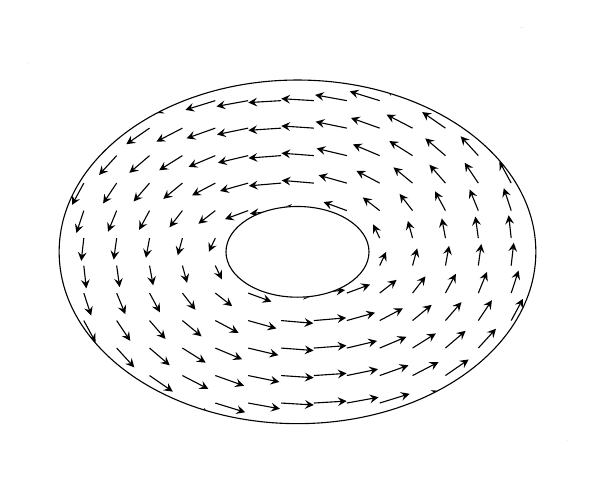
\begin{tikzpicture}[even odd rule]
%  \draw[rounded corners=35pt] (6.5,-1.8)--(2,-2)--(0,0) -- (2,2)--(4.2,1.4)--cycle;
%  \draw (3.5, 0.2) arc (-20:-130:0.9 and 0.7);
%  \draw (2.3, -0.15) arc (180:40:0.6 and 0.3);
%
%  \draw[thick, ->] (1.1, 0)--(1.4, 0.6);
%  \draw[thick, ->] (1.5, -0.6)--(1.6, 0.2);
%  \draw[thick, ->] (1.2, 0.8)--(2, 1.4);
%  \draw[thick, ->]  

\begin{axis}[%
  view     = {0}{90}, % for a view 'from above'
  domain   = -3:3,
  y domain = -3:3,
  %xtick    = {-3,...,3},
  %ytick    = {-3,...,3},
  axis line style={draw=none},
  ticks=none
  %tick style={draw=none}
]
\addplot3[
        quiver = {
            u = {-y/sqrt(x^2+y^2)},
            v = {x/sqrt(x^2+y^2+3)},
            scale arrows = 0.4,
        },
        -stealth,
        domain = -3:3,
        domain y = -3:3,
        samples=16
    ] {0};
%\addplot3[blue, quiver={u=8*x, v=2*y, scale arrows=0.05}, samples=16, -latex] (x,y,0);

  %\fill[clip, overlay=false, fill=white, color=white, fill opacity=0.5] (-4, 3.5) rectangle (5, -3.5) ellipse (0, 0) (1 and 0.5);

  \fill[preaction={clip}, fill=white] (-4,-3.5) rectangle (4,3.5) (0,0) ellipse (2.9 and 2.5);
  \draw (0,0) ellipse (2.9 and 2.5);
  \filldraw[white] (0,0) ellipse (0.84 and 0.66);
  \draw (0,0) ellipse (0.87 and 0.66);
 
\end{axis}
\end{tikzpicture}
\end{center}

Wyraźmy pole wektorowe $X:M\to TM$ w mapach $(U,\phi)$ na $M$ oraz $(TU,\overline{\phi})$ na $TM$. Niech $a_i:\phi(U)\to\R$ będą gładkimi funkcjami rzeczywistymi (nazwiemy je \acc[i]{współrzędnymi $X$} w mapach $\phi$ i $\overline{\phi}$) takimi, że
$$\overline{\phi}X\phi^{-1}(x)=(\;x,\;a_1(x),...,a_n(x)\;)=(\;x,\;\sum a_i(x)e_i\;),$$
gdzie $e_i$ to baza standardowa $\R^n$. Zgodnie z oznaczeniem z poprzedniego rozdziału $\frac{\partial}{\partial \phi_i}(p)=(\phi^*_p)^{-1}(e_i)$ mamy
$$X(p)=\sum a_i(\phi(p))\cdot\frac{\partial}{\partial\phi_i}(p).$$
Jeśli teraz oznaczymy $b_i=a_\circ\phi:U\to\R$, to wówczas
$$X(p)=\sum b_i(p)\cdot\frac{\partial}{\partial\phi_i}(p).$$

\begin{fact}
  Pole $X:M\to TM$ jest gładkim polem wektorowym na $M$ $\iff$ w mapaie $(U,\phi)$ na $M$ i odpowiadającej jej mapie $(TU,\overline{\phi})$ na $TM$ wyraża się jako
  $$X(p)=\sum b_i(p)\cdot\frac{\partial}{\partial\phi_i}(p)$$
  dla pewnych gładkich $b_i:U\to\R$.
\end{fact}

\begin{proof}
  Bezpośrednio z przestawienia $X$ w mapach $(U,\phi)$ i $(TU,\overline{\phi})$ jak wyżej.
\end{proof}

Pole wektorowe na otwartym $U\subseteq\R^n$ ma postać
$$X(x)=\sum_{i\leq n}a_i(x)\cdot\frac{\partial}{\partial x_i}(x)$$
dla pewnych gładkich funkcji $a_i:U\to\R$. Z tego powodu będziemy pisać
$$X(x)=[a_1(x),...,a_n(x)]\in \R^n\cong T_xU.$$
Zjawiska lokalne dla pól na rozmaitościach będziemy wyrażać za pośrednictwem map za pomocą pól na otwartych podzbiorach $\R^n$.

\begin{conclusion}\label{wniosek 5:3}
  Suma dwóch gładkich pól wektorowych
  $$(X+Y)(p):=X(p)+Y(p)$$
  jest gładkim polem wektorowym.

  Iloczyn gładkiej funkcji $f:M\to\R$ oraz gładkiego pola $X$
  $$(f\cdot X)(p):=f(p)\cdot X(p)$$
  jest gładkim polem wektorowym
\end{conclusion}

Rodzinę wszystkich gładkich pól wektorowych na $M$ będziemy oznaczać przez $C^\infty(TM)$ lub $\color{blue}\mathfrak{X}(M)$. W algebraicznym rozumienia jest to moduł nad pierścieniem $C^\infty(M)$ gładkich funkcji rzeczywistych na $M$ (patrz wniosek \ref{wniosek 5:3}).

\subsection{Definiowanie pola wektorowego za pomocą rozkładów jedności}

Niech $M$ będzie rozmaitością z niepustym brzegiem $\partial M$. 

\begin{definition}
  Mówimy, że wektor $Y\in T_pM$, gdzie $p\in\partial M$, jest \important{skierowany do wewnątrz} $M$, jeśli w pewnej mapie $\phi:U_p\to H^n$ wyraża się przez
  $$Y=\sum_{i\leq n}a_i\cdot\frac{\partial}{\partial\phi_i}(p),\quad a_n>0$$
\end{definition}

\begin{fact}
  Jeśli wektor o początku $p$ jest skierowany do wewnątrz w jednej mapie, to jest tak w każdej innej mapie wokół $p$. Ponadto, suma wektorów skierowanych do wewnątrz jest wektorem skierowanym do wewnątrz.
\end{fact}

\begin{proof}
  Niech $Y$ będzie wektorem skierowanym do wewnątrz w mapie $(U,\phi)$. Niech $(V, \psi)$ będzie inną mapą wokół $p$. Wiemy, że
  $$Y=\sum a_i\cdot\frac{\partial}{\partial\phi_i}(p)$$
  i $a_n>0$. Chcemy teraz sprawdzić, co się dzieje w indeksie $n$, gdy przedstawimy ten wektor jako kombinację liniową $\frac{\partial}{\partial\psi_i}(p)$. Popatrzmy na zamianę baz:
  \begin{align*}
    \frac{\partial}{\partial\phi_n}(p)&=(\phi^*_p)^{-1}(e_n)=\\
        &=(\psi_p^*)^{-1}[\psi_p^*(\phi_p^*)^{-1}](e_n)=\\
        &=(\psi_p^*)^{-1}d\psi_p d(\phi)^{-1}_{\phi(p)}(e_n)=\\
        &=(\psi_p^*)^{-1}[d(\psi\phi^{-1})_{\phi(p)}(e_n)]
  \end{align*}
  Wiemy, że $\psi\phi^{-1}:\R^n\to\R^n$ jest funkcją rzeczywistą, czyli 
  $$d(\psi\phi^{-1})_{\phi(p)}=D_{\phi(p)}(\psi\phi^{-1})$$
  jest jej pochodną. Dodatkowo, wiemy, że $\psi\phi^{-1}$ jest bijekcją, więc na pewno $D_{\phi(p)}(\psi\phi^{-1})(e_n)$ nie może się zerować. Zarówno $\psi$ jak i $\phi$ są mapami wokół brzegu $\partial M$, czyli tak naprawdę:
  $$\psi\phi^{-1}:H^n\to H^n$$
  W takim razie, $D_{\phi(p)}(\psi\phi^{-1})(e_n)>0$ i mamy
  $$a_n\cdot\frac{\partial}{\partial\phi_n}(p)=\underbrace{a_n\cdot D_{\phi(p)}(\phi\psi^{-1})(e_n)}_{>0}\cdot\frac{\partial}{\partial\psi_n}$$
  

  %więc $Y$ zapisane w bazie $\frac{\partial}{\partial\psi_n}$ma ściśle dodatnią ostatnią współrzędną.

  Dla sumy wektorów $X+Y$ takich, że $X=\sum a_i\frac{\partial}{\partial\phi_i}(p)$ i $Y=\sum b_i\frac{\partial}{\partial\phi_i}(p)$, $a_n,b_n>0$, mamy
  $$X+Y=\sum(a_i+b_i)\frac{\partial}{\partial\phi_i}(p)$$
  więc $a_i+b_i>0$.
\end{proof}

\begin{definition}
  Pole wektorowe $X:M\to TM$ jest \important{skierowane do wewnątrz} $M$, jeśli dla każdego $p\in\partial M$ $X(p)$ jest skierowany do wewnątrz $M$.
\end{definition}

\begin{fact}
  Na każdej rozmaitości gładkiej z brzegiem $M$ istnieje gładkie pole wektorowe $X$ skierowane do wewnątrz $M$.
\end{fact}

\begin{proof}
  Rozważmy rozkład jedności $\{f_i\}$ wpisany w pokrycie $M$ zbiorami mapowymi $U_\alpha$ i niech $supp(f_i)\subseteq U_{\alpha_i}$. Dla tych $U_\alpha$, które zahaczają o brzeg $\partial M$ określmy pola wektorowe
  $$X_\alpha:U_\alpha\to TU_\alpha\subseteq TM$$
  $$X_{\alpha}(p)=\frac{\partial}{\partial(\phi_\alpha)_n}(p).$$
  Dla pozostałych $U_\alpha$ określamy $X_\alpha$ dowolnie.

  \begin{figure}[h!]
    \begin{illustration}
      \filldraw[orange!20] (7.5, 0.25) arc (20:340:1 and 0.5);
      \draw[rounded corners=35pt](7,-1)--(4.2,-1)--(2,-2)--(0,0) -- (2,2)--(4.2,1)--(7,1);
      \draw (1.5,0.2) arc (175:315:1cm and 0.5cm);
      \draw (3,-0.28) arc (-30:180:0.7cm and 0.3cm);
      \filldraw[color=black, fill=blue!40!black!60] (7.5,0) arc (0:360:0.5cm and 1cm);

      \filldraw[orange!20] (8.5, 0) arc (180:0:1 and 1.3);
      \draw (8, 0)--(11, 0);
      \draw (9.5, 0)--(9.5, 1.5);

      \node at (6.5, 1.4) {$U_\alpha$};
      \node at (11, 0.5) {$\frac{\partial}{\partial x_n}$};
      \path (6.4, 1.2) edge [bend right=20] (6.3, 0.4);
      \path[->] (6, -0.2) edge [bend right=30] node [midway, below] {$\phi_\alpha$} (9, -0.3);
    \end{illustration}
  \end{figure}
  Zdefiniujmy teraz pole wektorowe:
  $$X=\sum_jf_jX_{\alpha_j},$$
  które jest lokalnie skończoną kombinacją gładkich pól skierowanych do wewnątrz i funkcji dodatnich. Jest to więc pole wektorowe skierowanie do wewnątrz.
\end{proof}

\subsection{Przenoszenie gładkich pól wektorowych przez dyfeomorfizmy}

Niech $f:M\to N$ będzie dyfeomorfizmem i niech $X\in\mathfrak{X}(M)$ będzie gładkim polem wektorowym na $M$. Poszczególne wektory $X_p$ pola $X$ przenoszone przez odwzorowanie styczne $df$ do $TN$ tworzą pola wektorowe na $N$ oznaczane przez $df(X)$ w ten sposób, że
$$\color{blue}df_p(X_p)=df(X)_{f(p)}.$$
Określamy pole wektorowe $df(X)$ na $N$ przez
$$df(X)_q:=df_{f^{-1}(q)}(X_{f^{-1}(q)})\in T_qN\subseteq N.$$
Powyższe określenia oznaczają, że pole $df(X)$, jako odwzorowanie $N\to TN$, jest złożeniem
$$\color{blue}df(X)=df\circ X\circ f^{-1}.$$
Jako złożenie odwzorowań gładkich, samo też jest odwzorowaniem gładkim.

\begin{definition}
  Gładkie pole wektorowe $df(X)$ określone jak wyżej jest nazywane \important{przeniesieniem} pola $X$ na $N$ przez dyfeomorfizm $f$.
\end{definition}

  Jeśli o dyfeomorfiźmie $f$ myślimy jako o sposobie utożsamienia rozmaitości $M$ i $N$, to o polu $df(X)$ na $N$ możemy myśleć jako o tym samym polu co pole $X$ na $M$ względem utożsamienia za pomocą $f$.

\begin{example}
  \item Wybierzmy pole $X\in\mathfrak{X}(M)$, takie, że dla mapy $(U,\phi)$ na $M$ mamy
    $$X(p)=\sum a_i(p)\cdot\frac{\partial}{\partial\phi_i}(p),\quad p\in U.$$
    Wówczas
    \begin{itemize}
      \item przeniesienie pola $X\restriction U$ na $\phi(U)$ przez dyfeomorfizm $\phi$ daje pole $d\phi(X)(u)=\sum a_i(\phi^{-1}(u))\cdot\frac{\partial}{\partial x_i}(x)$
      \item wyrażenie pola $X$ w mapach $(U,\phi)$ na $M$ oraz $(TU,\overline{\phi})$ na $TM$ daje
        $$\overline{\phi}X\phi^{-1}(x)=(\;x,\;a_1(\phi^{-1}(x)),...,a_n(\phi^{-1}(x))\;)$$
    \end{itemize}
    Oba te pola, a zwłaszcza pierwsze z nich, będziemy nazywać \acc[b]{wyrażeniem pola $X$}\marginpar{Dowód w lemacie \ref{lemat:5.10}} w mapie $(U,\phi)$. Ponadto zachodzi
    $$X(p)=[c,t_0]\iff d\phi(X)(\phi(p))=[\phi\circ c, t_0]$$
\end{example}

\subsection{Krzywe całkowe}

\begin{definition}
  Niech $M$ będzie rozmaitością bez brzegu. \important{Krzywą całkową} pola wektorowego $X\in\mathfrak{X}(M)$ to dowolna krzywa
  $$\gamma:(a,b)\to M$$
  taka, że dla każdego $t\in (a,b)$
  $$\gamma'(t)=[\gamma, t]=X(\gamma(t))$$
\end{definition}

\begin{lemma}\label{lemat:5.10}
  Niech $\gamma$ będzie krzywą całkową pola $X\in\mathfrak{X}(M)$ $\iff$ dla każdej mapy $(U,\phi)$ na $M$ krzywa $\phi\circ\gamma$ jest krzywą całkową pola $d\phi(X)\in\mathfrak{X}(\phi(U))$.
\end{lemma}

\begin{proof}$ $\newline

  $\implies$

  Jeśli $\gamma'(t)=[\gamma,t]=X_{\gamma(t)}$, to z definicji $d\phi$ mamy 
\reversemarginpar\marginpar{Dla przypomnienia: $df(X)_{f(p)}=df_p(X_p)$}
  $$(\phi\circ\gamma)'(t)=[\phi\circ\gamma,t]=d\phi_{\gamma(t)}([\gamma,t])=d\phi(X_{\gamma(t)})=d\phi(X)_{\phi\circ\gamma(t)}$$

  $\impliedby$

  Niech $(\phi\circ\gamma)'(t)=[\phi\circ\gamma,t]=d\phi(X)_{\phi\circ\gamma(t)}$. Wówczas
  \begin{align*}
    \gamma'(t)&=[\phi^{-1}(\phi\circ\gamma)]'(t)=d\phi^{-1}_{ \phi\circ\gamma(t)}[ (\phi\circ\gamma)'(t)]=\\
              &=d\phi_{\phi\circ\gamma(t)}[d\phi(X)_{\phi\circ\gamma(t)}]= \underbrace{d\phi^{-1}_{\phi\circ\gamma(t)}d\phi_{\gamma(t)}}_{id_{T_{\gamma(t)}M}}(X_{\gamma(t)})=X_{\gamma(t)}
  \end{align*}
\end{proof}

\begin{theorem} Dla \marginpar{Krzywe całkowe wyrażenia pola $X$ w mapie $(U,\phi)$ to wyrażenie krzywych całkowych pola $X$ w tej samej mapie.}każdego $p\in M$ istnieje krzywa całkowa o początku w $p$, tzn. krzywa całkowa $\gamma:(-\epsilon,\epsilon)\to M$ taka, że $\gamma(p)=p$
\end{theorem}

\begin{proof}
\end{proof}
